This chapter first discusses the experiments carried out in order to both improve the performance, and gain a better understanding, of the sub-components implemented. Experiments such as hyperparameter optimisation and ablation studies including both the two dimensional and three dimensional models are discussed. Once the results are cross-validated, the final results achieved by the optimised models resulting from the experimentation are then presented, interpreted, and compared to results achieved by alternative models. Finally, various aspects of the project are critically evaluated.

\section{Two Dimensional Experimentation}

This section reintroduces the initial results achieved by the ``baseline'' 2D model implemented in Chapter \ref{chap:implementation} and then outlines the experiments carried out in an attempt to improve the performance both qualitatively and quantitatively.

\subsection{Initial Results}

\begin{figure}[!b]
    \begin{subfigure}[b]{0.49\textwidth}
        \centering
        \begin{tikzpicture}[scale=0.9]
            \begin{axis}[
                height=\axisdefaultheight,
                ylabel=\small{Loss},
                xlabel=\small{Epochs},
                grid=major,
                legend pos=north east,
                legend cell align=left,
                legend style={fill=white, fill opacity=0.8, draw=none,text opacity=1}]
                \addplot[blue, mark=x] table [x=xs, y=tl, col sep=comma] {csv/base.csv};
                \addlegendentry{\small{Train Loss}}
                \addplot[magenta, mark=x] table [x=xs, y=vl, col sep=comma] {csv/base.csv};
                \addlegendentry{\small{Val Loss}}
            \end{axis}
        \end{tikzpicture}
        \caption{Loss curve}
    \end{subfigure}
    \hfill
    \begin{subfigure}[b]{0.49\textwidth}
        \centering
        \begin{tikzpicture}[scale=0.9]
            \begin{axis}[
                height=\axisdefaultheight,
                ylabel=\small{Accuracy (\%)},
                xlabel=\small{Epochs},
                grid=major,
                legend pos=south east,
                legend cell align=left,
                legend style={fill=white, fill opacity=0.8, draw=none,text opacity=1}]
                \addplot[blue, mark=x] table [x=xs, y=ta, col sep=comma] {csv/base.csv};
                \addlegendentry{\small{Train Accuracy}}
                \addplot[magenta, mark=x] table [x=xs, y=va, col sep=comma] {csv/base.csv};
                \addlegendentry{\small{Val Accuracy}}
            \end{axis}
        \end{tikzpicture}
        \caption{Loss curve}
    \end{subfigure}
    \caption{The loss and accuracy curves achieved when training the model over 20 epochs using the hyperparameters outlined in Table \ref{tab:initialhyperparams}.}
    \label{fig:basetrainacc}
\end{figure}

\begin{figure}[!t]
    \centering
    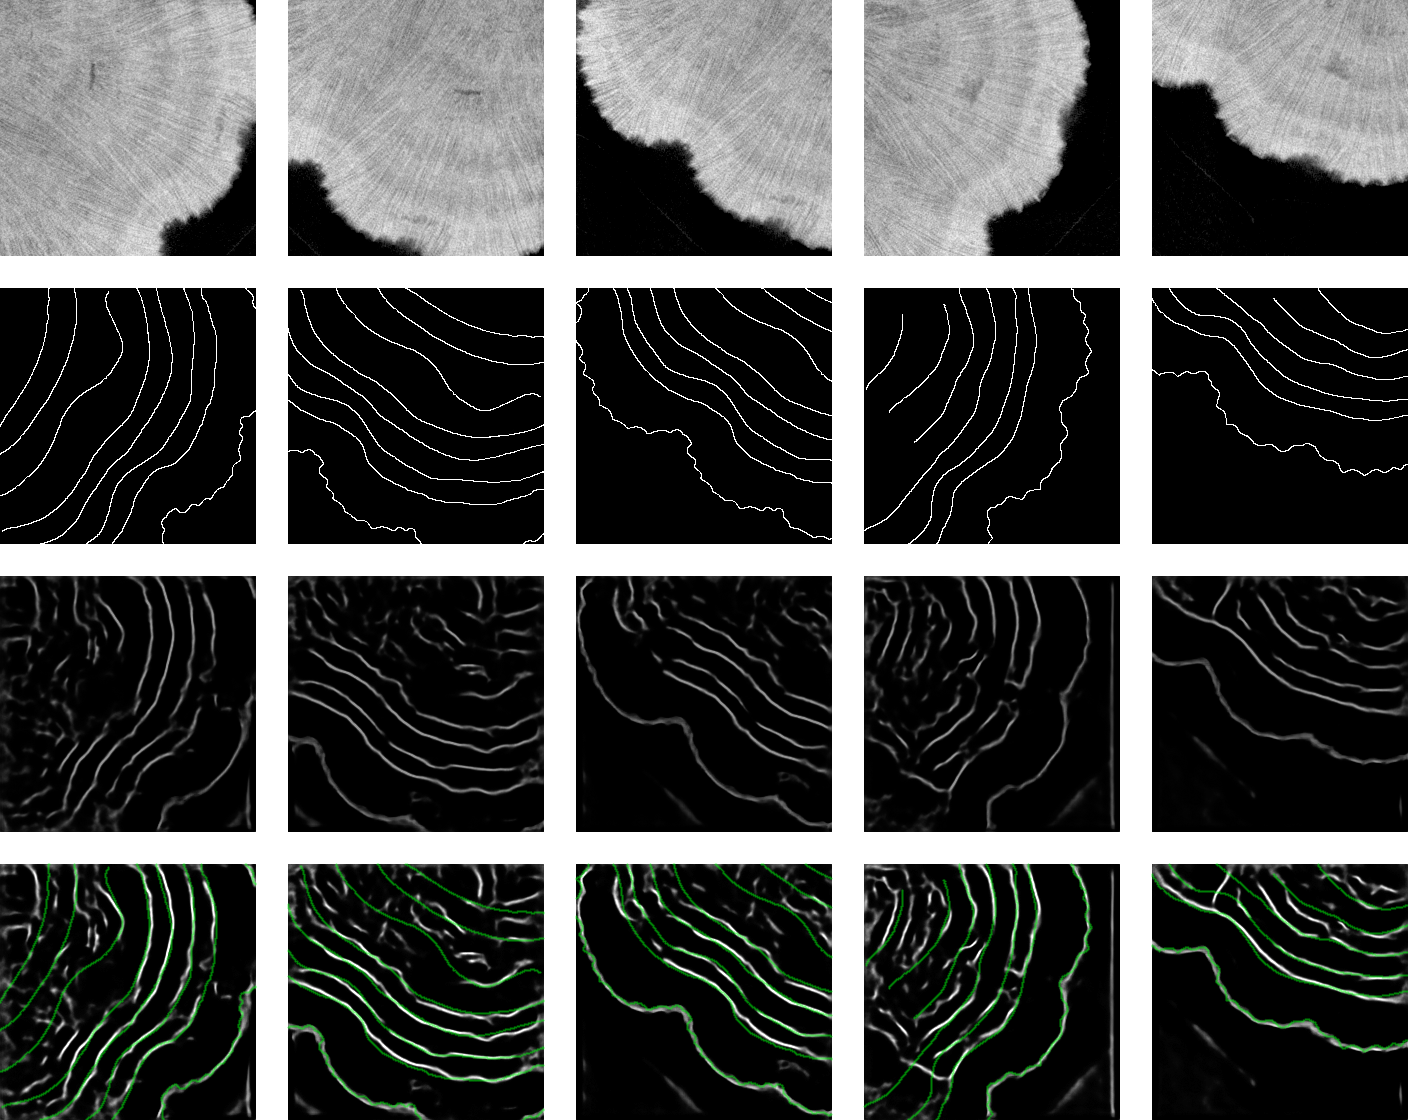
\includegraphics[width=1\textwidth]{images/initial-outputs.png}
    \caption{Good and bad results placeholder.}
    \label{fig:goodbad}
\end{figure}

The initial results achieved by the baseline model can be discussed further in order to gain a better understanding of the strengths and weaknesses of the model. The loss and accuracy curves are shown in Figure \ref{fig:basetrainacc} and example boundary predictions of both high and low ``quality'' are shown in Figure \ref{fig:goodbad}. Their quality is assessed both via the accuracy metric achieved and via visual inspection. Looking at Figure \ref{fig:basetrainacc}, it can be see that the accuracy achieved on the validation set is noticeably lower than the accuracy achieved on the training set. This unusual behaviour may be due to the validation set containing ``easier'' examples in which the annual banding is more obvious. Although the performance reported on this validation set may potentially be positively skewed, the final performance achieved by the model will be reported on cross-validated results and so the selection biases that arise from this dataset split should not affect the final reported performance.

\subsection{Hyperparameter optimisation}

As discussed in Chapter \ref{chap:technical}, the performance achieved by deep neural networks is known to depend critically on the identification of a good set of hyperparameters~\cite{hyperparam, goodhyperparam}. In this project, a manual form of grid search was used to discover the optimal set of hyperparameter configurations. In this technique, all hyperparameters are fixed and only a single hyperparameter is varied at a time. Although this may not be the most efficient approach, it enables a better understanding of the model to be gained.

% Due to the time constraints of the project, it would not be possible to perform an exhaustive search of all possible hyperparameter configurations. Thus, the primary aim of this chapter is not to achieve the best performance possible, but instead to evaluate which hyperparameters affect the performance most and reason as to why this is the case.

\subsubsection{Learning Rate}

Of all the hyperparameters relevant to deep learning models, the optimisation of the learning rate often has the biggest impact on the performance of a model~\cite{bengio2012practical}. The selection of a learning rate too large can cause an optimisation algorithm to take a step ``over'' minima causing the loss to inadvertently increase rather than decrease. The selection of a learning rate too small can also hinder performance as the optimisation algorithm may become permanently stuck in a suboptimal local minimum~\cite{goodfellow}.

Since it is usually not possible to calculate an optimal learning rate a priori~\cite{neuralbook}, some form of trial and error is required. A reasonable range of values to experiment with are given by Bengio in~\cite{bengio2012practical} and will be used as the basis of the values experimented with in this section. Bengio suggests an initial learning rate within the range of $10^{-6}$ to $1$.

The accuracies achieved when training the network using various initial learning rates in this range are shown in Figure \ref{fig:lrplot}. It can be seen that the final average accuracy achieved after 20 epochs is similar for all but the 0.00001 value. Although it may look like the accuracy for this learning rate could still improve with further training, the accuracy does not improve further even after 40 epochs. This plateau in the accuracy achieved suggests that the 0.00001 learning rate may be low enough to become stuck in suboptimal local minima.

The training loss achieved by the 0.001 learning rate oscillated at ${\sim}0.5$ for the entire training process, even over multiple training attempts. In comparison, the 0.00005 learning rate achieved a training loss of 0.06 and a validation loss of 0.16. These oscillations are a common sign of a learning rate being too high and stepping ``over'' minima~\cite{bishop1995neural}. Pure black images were output for all samples in both the training and validation set resulting in an accuracy of 0\% being achieved.

Although the both the 0.00005 and 0.0001 learning rates all achieved a similar accuracy of ${\sim}96\%$ after 20 epochs, the 0.00005 value was ultimately chosen for multiple reasons. First, the accuracy curve is smoother than the curves resulting from higher values, allowing the accuracy to be more reliably used as a stopping criteria for early stopping. Second, when inspecting the results visually, the 0.00005 learning rate results in predictions that are far clearer in the inner areas of the coral skeleton than any other learning rate. Although most of the learning rates were able to produce acceptable predictions nearer to the surface of the coral, only the 0.00005 learning rate was able to produce acceptable predictions in these inner areas. An example of a patch that benefitted from the 0.00005 learning rate is shown in Figure \ref{fig:lrdiff}.

\begin{figure}[!t]
    \begin{subfigure}[b]{0.49\textwidth}
        \centering
        \begin{tikzpicture}[scale=0.9]
            \begin{axis}[
                height=\axisdefaultheight,
                ylabel=\small{Accuracy (\%)},
                xlabel=\small{Epochs},
                grid=major,
                legend pos=south east,
                legend cell align=left,
                legend style={fill=white, fill opacity=0.8, draw=none,text opacity=1}]
                \addplot[magenta, mark=x] table [x=xs, y=lr00001_vacc, col sep=comma] {csv/lr.csv};
                \addlegendentry{\small{$\eta=0.00001$}}
                \addplot[darkgray, mark=x] table [x=xs, y=lr00005_vacc, col sep=comma] {csv/lr.csv};
                \addlegendentry{\small{$\eta=0.00005$}}
                \addplot[blue, mark=x] table [x=xs, y=lr0001_vacc, col sep=comma] {csv/lr.csv};
                \addlegendentry{\small{$\eta=0.0001$}}
                \addplot[orange, mark=x] table [x=xs, y=lr0005_vacc, col sep=comma] {csv/lr.csv};
                \addlegendentry{\small{$\eta=0.0005$}}
            \end{axis}
        \end{tikzpicture}
        \caption{Varying learning rate}
        \label{fig:lrplot}
    \end{subfigure}
    \hfill
    \begin{subfigure}[b]{0.49\textwidth}
        \centering
        \begin{tikzpicture}[scale=0.9]
            \begin{axis}[
                height=\axisdefaultheight,
                ylabel=\small{Accuracy (\%)},
                xlabel=\small{Epochs},
                grid=major,
                legend pos=south east,
                legend cell align=left,
                legend style={fill=white, fill opacity=0.8, draw=none,text opacity=1}]
                \addplot[magenta, mark=x] table [x=xs, y=bs1_vacc, col sep=comma] {csv/batch.csv};
                \addlegendentry{\small{$batch=1$}}
                \addplot[darkgray, mark=x] table [x=xs, y=bs2_vacc, col sep=comma] {csv/batch.csv};
                \addlegendentry{\small{$batch=2$}}
                \addplot[blue, mark=x] table [x=xs, y=bs4_vacc, col sep=comma] {csv/batch.csv};
                \addlegendentry{\small{$batch=4$}}
                \addplot[teal, mark=x] table [x=xs, y=bs8_vacc, col sep=comma] {csv/batch.csv};
                \addlegendentry{\small{$batch=8$}}
                \addplot[orange, mark=x] table [x=xs, y=bs16_vacc, col sep=comma] {csv/batch.csv};
                \addlegendentry{\small{$batch=16$}}
            \end{axis}
        \end{tikzpicture}
        \caption{Varying batch size}
        \label{fig:bsplot}
    \end{subfigure}
    \caption{The accuracies achieved on the validation set using various hyperparameter values. A TensorBoard smoothing value of 0.3 was used. \textbf{(left)} The accuracies achieved when training the network using various initial learning rate values $\eta$. Apart from the learning rate, the same hyperparameters used to achieve the initial results (outlined in Table \ref{tab:initialhyperparams}) were used once again. \textbf{(right)} The accuracies achieved when training the network using various batch sizes. Apart from a learning rate of 0.00005 being used, the hyperparameters outlined in Table \ref{tab:initialhyperparams} were used once again.}
\end{figure}

\begin{figure}[!t]
    \includegraphics[width=\textwidth, height=0.6\textwidth]{example-image-a}
    \caption{0.0001 vs 0.00005 examples.}
    \label{fig:lrdiff}
\end{figure}

\subsubsection{Batch Size}

The next parameter experimented with was the batch size. Ranging from anywhere from a size of one up to even a few hundreds in some applications~\cite{bengio2012practical}, the batch size is a parameter 

Values in the range of one to 16 were experimented with. The accuracies achieved when training using these various batch sizes are shown in Figure \ref{fig:bsplot}. Note that in order to ensure that the model was exposed to the same number of samples per epoch, with each increase in batch size, the \texttt{steps-per-epoch} argument of the \texttt{fit} method was also decreased. For example, if the batch size was doubled, the \texttt{steps-per-epoch} was halved.

Values above 16 were not experimented with as the accuracy achieved was decreasing as the batch size increases. 

with each increase in batch size, decrease no of steps per epoch so that the number of samples seen in the end is the same (since steps per epoch specifies the number of batches per epoch, not samples).

unet paper uses 1? 2? sensible ranges are??

try batch sizes 1, 2, 4, 8, 16, 32, 64, 128?

bengio does say that learning rate and batch size should be reoptimised at the end

``With an increase in the number of nodes, the batch size grows. But trainingwith large batch size often results in the lower model accuracy.'': \url{https://arxiv.org/pdf/1708.03888.pdf}

Also in paper above: on page 3 they show table of training alex net with different batch sizes and show that accuracy decreases with increasing batch size.

``it has been observed in practice that when using a larger batch there is a degradation in the quality of the model, as measured by its ability to generalize.'': \url{https://arxiv.org/pdf/1609.04836.pdf}

``It is often better to use a larger batch size so a larger learning rate can be used.'': \url{https://arxiv.org/pdf/1803.09820.pdf}

\subsubsection{Optimisation Algorithms}

Said in tech bg that I experimented with diff optimisers so need to add comparisons to SGD etc.

Look at the momentum values of adam? play around a little?

Tried SGD with 0.00005, 0.0001, 0.0005, no good results. maybe example output image? maybe the momentum of adam was very important? loss stuck at 0.16 and val loss never came below 0.3. Very similar results for adam with epsilon=1 and epsilon=? maybe suggests that the epsilon (maybe explain what adam say epsilon does?) is very important for the performance of adam?

\subsubsection{Loss Functions}

\begin{figure}[!t]
    \includegraphics[width=\textwidth, height=0.6\textwidth]{example-image-b}
    \caption{Focal loss examples vs cross-entropy loss examples.}
    \label{fig:lossfunctiondiff}
\end{figure}

Focal loss and other loss functions? to combat class imbalance

Look at the alpha and gamma values of focal loss? play around with them a little. look at the table in the original paper that says when you should use what.

At the end of this section, resummarise the configuration of chosen params now in Table \ref{tab:hyperparams1}.

\begin{table}[t]
    \centering
    \caption{A summary of the initial hyperparameter settings used.}
    \begin{tabular}{@{}ll@{}}
    \toprule
    Hyperparameter   & Setting      \\ \midrule
    Architecture     & 2D U-Net   \\
    Optimiser & Adam \\
    Learning rate & 0.00005 \\
    Loss function & Cross-entropy \\
    Epochs & 20 \\
    Steps per epoch & 500 \\
    Batch size & 2 \\ \bottomrule
    \end{tabular}
    \label{tab:hyperparams1}
\end{table}

\subsubsection{Dropout}

REMEMBER TO TRY AND UNDERSTAND WHY WHAT EVER HAPPENS IS THE CASE AND BACK IT UP ALL THROUGHOUT

vary from 0.1 to 0.9? same with spatial

\subsubsection{Spatial Dropout}

Need to talk about dropout? maybe only mention it in evaluation?
Spatial drop out better for fully conv? \url{https://arxiv.org/pdf/1411.4280.pdf}

% From Keras docs I think
% This version performs the same function as Dropout, however it drops
% entire 2D feature maps instead of individual elements. If adjacent pixels
% within feature maps are strongly correlated (as is normally the case in
% early convolution layers) then regular dropout will not regularize the
% activations and will otherwise just result in an effective learning rate
% decrease. In this case, SpatialDropout2D will help promote independence
% between feature maps and should be used instead.

\subsubsection{Kernel Sizes}

\subsubsection{L2 Regularization}

\subsection{Resolution}

\subsection{Augmentation}
\label{sec:evalaugmentation}

\subsubsection{No Augmentation}

\subsubsection{Augmentation Ranges}

\subsection{Ablation Studies}

comparison of convtranspose to upsample and then conv.

remove the relu at the end of the implementation?

Maybe visualise ablations with a graph showing each ablation with accuracy achieved or something? like in that paper. or a table?

\section{Three Dimensional Experimentation}

\subsection{Hyperparameter optimisation}

Due to the time constraints of the project, far fewer hyperparameters were optimised for the three dimensional architectures.

Briefly mention that various learning rates and batch sizes were experimented with but none produced better results (unless then do?) and the new optimal hyperparameters for the 2D arch were used.

\subsection{Augmentation}

\subsection{Alternative Modified Architectures}

Varying numbers of output channels in Conv3D layers as you said youd experiment with this.

\subsection{Fully Three Dimensional Architecture}

\subsubsection{Data}

Lack of data. Was not consistently labelled. Show adjacent slices. Proves how hard it is to label images.

\section{Cross-validation}
\label{sec:evalcrossval}

\subsection{Train/test Splits}

\section{Final Results}

\begin{figure}[!p]
    \centering
    \includegraphics[width=\textwidth, height=1.45\textwidth]{example-image-b}
    \caption{A full page of final results achieved.}
    \label{fig:finalresults}
\end{figure}

\section{Comparisons with Other Architectures}

Compare SegNet, U-Net, pix2pix. Maybe find somewhere to put in the pix2pix generation for fun? If not don't worry. Do mention pix2pix using different backbones or whatever its called and why you think it didnt perform well.

\subsection{SegNet}

\subsection{pix2pix}

\section{Critical Evaluation}

\subsection{Boundary Extraction}

\subsubsection{Labelling}

\subsubsection{Lack of Data}

very hard for a non expert to label.

\subsection{Accuracy Metric}

Can't tell which boundary it should be looking for. a completely white image would produce 100\% accuracy but the skeletonization makes the amount of white pixels low.

Maybe show concrete examples of where it falls down? images shifted to the right so that one boundary is roughly where another should be? images that have many white lines that are even perpendicular to the right labels should still produce a pretty low score?

Show image produced by SGD. completely wrong but still gets 60\% due to the white part in the bottom left of the image.

visual inspection is still needed take for example the learning rate plots, they all achieve accuracies within a percentage of each other but some are clearly worse than others?

\subsection{Calcification Rate Estimation}

\section{Comparisons with Existing Techniques}

Erica sent a paper a while ago that used a computer program to calculate the calcification rate  \url{https://www.geosociety.org/datarepository/2015/2015015.pdf} check the email from her with subject DeCarlo Paper

% {\bf A topic-specific chapter, of roughly $15$ pages} 
% \vspace{1cm} 

% \noindent
% This chapter is intended to evaluate what you did.  The content is highly 
% topic-specific, but for many projects will have flavours of the following:

% \begin{enumerate}
% \item functional  testing, including analysis and explanation of failure 
%       cases,
% \item behavioural testing, often including analysis of any results that 
%       draw some form of conclusion wrt. the aims and objectives,
%       and
% \item evaluation of options and decisions within the project, and/or a
%       comparison with alternatives.
% \end{enumerate}

% \noindent
% This chapter often acts to differentiate project quality: even if the work
% completed is of a high technical quality, critical yet objective evaluation 
% and comparison of the outcomes is crucial.  In essence, the reader wants to
% learn something, so the worst examples amount to simple statements of fact 
% (e.g., ``graph X shows the result is Y''); the best examples are analytical 
% and exploratory (e.g., ``graph X shows the result is Y, which means Z; this 
% contradicts [1], which may be because I use a different assumption'').  As 
% such, both positive {\em and} negative outcomes are valid {\em if} presented 
% in a suitable manner.